\documentclass{scrreprt}

\usepackage{amsmath}
\usepackage[margin=0.8in]{geometry}
\usepackage{graphics}
\usepackage{graphicx}
\usepackage[round]{natbib}
\usepackage{pst-node}
\bibliographystyle{plainnat}

\title{Evapotranspiration Modeling in ECHSE: Documentation}
\author{Julius Eberhard}

%--------------------------------------------------------------------------------
%--------------------------------------------------------------------------------

\begin{document}

\maketitle
\tableofcontents

%--------------------------------------------------------------------------------

\chapter{Introduction} \label{ch:introduction}

This is a documentation of my work done in exploring some aspects of the way how evapotranspiration is simulated in the \emph{Eco-Hydrological Simulation Environment} (ECHSE, \citealt{kneis15}) with methods, classes, and engines written by Tobias Pilz.
ECHSE is a model framework, i.e. a software providing calculation methods that can be composed modularly to form model engines. These engines can be compiled and be run as independent models with input data.
ECHSE is used in the field of (eco-)hydrology and therefore comes with a collection of methods especially relevant for issues in this field.
The goal of the bigger project is to apply with ECHSE different ways of determining the potential ($et_{pot}$) and the actual evapotranspiration ($et_{act}$).
These are, as of the date of this documentation:
\begin{itemize}
  \item[--] the simple model of \citet{makkink57},
  \item[--] the equation of Penman \& Monteith \citep{monteith65},
  \item[--] the FAO Penman-Monteith equation (``reference evaporation''),
  \item[--] the equation of Shuttleworth \& Wallace \citep{shuttleworth85}.
\end{itemize}

The engine-specific names of variables and parameters are written in \verb!fixed-width! whereas the physical symbols of variables, constants and parameters are written in \textit{italics}.
E.g., extraterrestrial radiation = $R_{ex}$ = \verb!radex!.
Terms that describe parts of the ECHSE architecture are written in \textsf{sans-serif}.

\section{Model overview -- parameter overview} \label{sec:intro_overview}

The engine parameters can be grouped into
\begin{itemize}
  \item[--] aerodynamic parameters,
  \item[--] geographical parameters,
  \item[--] radiation parameters,
  \item[--] soil hydraulic parameters,
  \item[--] vegetation parameters,
\end{itemize}
%
according to their physical role, and will be discussed in this order in chapter \ref{ch:parest}.
Within the ECHSE engines, parameters are grouped into the types
\begin{itemize}
  \item[--] \textsf{paramNum} (object-specific scalar parameters),
  \item[--] \textsf{sharedParamNum} (group-specific scalar parameters),
  \item[--] \textsf{inputExt} (group-specific time-dependent scalar parameters treated as external input variables),
\end{itemize}
%
according to their role in the computation process.
Tab. \ref{tab:varpar} contains an overview of the variables and parameters and whether they are used in the different $et$ models (Makk = Makkink, PM = Penman-Monteith, FAO = FAO Penman-Monteith, SW = Shuttleworth-Wallace model).
The parameters in this overview are grouped into the types \textsf{paramNum}, \textsf{sharedParamNum}.
Parameters of the \textsf{inputExt} type can be found together with the actual external input variables.

\begin{table}[ht]
  \caption{External input variables, parameters and their usage in the $et$ models.
           For abbreviations, see text.
           \textbullet: required by engine primarily, (\textbullet): required only in cases when primary input is missing.}
  \scalebox{0.7}{%
    \begin{tabular*}{0.70\hsize}{cccc|ccc|r}
      \hline
      \multicolumn{4}{c}{$et_{pot}$}                                & \multicolumn{3}{c}{$et_{act}$}  & \\
      Makk          & PM            & FAO           & SW            & PM          & FAO & SW          & ECHSE name \\
      \hline
                    &               &               &               &             &     &             & \textbf{\textsf{inputExt}} \\
                    & (\textbullet) & (\textbullet) & (\textbullet) &             &     &             & \texttt{alb} \\
      \textbullet   & \textbullet   & \textbullet   & \textbullet   &             &     &             & \texttt{apress} \\
                    & \textbullet   &               & \textbullet   &             &     &             & \texttt{cano\_height} \\
      (\textbullet) & (\textbullet) & (\textbullet) & (\textbullet) &             &     &             & \texttt{cloud}* \\
      (\textbullet) & (\textbullet) & (\textbullet) & (\textbullet) &             &     &             & \texttt{doy} \\
      \textbullet   & \textbullet   & (\textbullet) & \textbullet   &             &     &             & \texttt{glorad} \\
                    & (\textbullet) & (\textbullet) & (\textbullet) &             &     &             & \texttt{glorad\_max} \\
      (\textbullet) & (\textbullet) & (\textbullet) & (\textbullet) &             &     &             & \texttt{hour} \\
                    & \textbullet   &               & \textbullet   &             &     &             & \texttt{lai} \\
                    & (\textbullet) & (\textbullet) & (\textbullet) &             &     &             & \texttt{rad\_long} \\
                    & \textbullet   & \textbullet   & \textbullet   &             &     &             & \texttt{rad\_net} \\
                    & (\textbullet) & (\textbullet) & \textbullet   &             &     &             & \texttt{rad\_net\_soil} \\
                    & \textbullet   & \textbullet   & \textbullet   &             &     &             & \texttt{rhum} \\
                    & \textbullet   &               & \textbullet   &             &     &             & \texttt{soilheat} \\
      (\textbullet) & (\textbullet) & (\textbullet) & (\textbullet) &             &     &             & \texttt{sundur} \\
      (\textbullet) & (\textbullet) & (\textbullet) & (\textbullet) &             &     &             & \texttt{temp\_max} \\
      (\textbullet) & (\textbullet) & (\textbullet) & (\textbullet) &             &     &             & \texttt{temp\_min} \\
      \textbullet   & \textbullet   & \textbullet   & \textbullet   &             &     &             & \texttt{temper} \\
                    &               &               & \textbullet   &             &     &             & \texttt{totalheat} \\
      (\textbullet) & (\textbullet) & (\textbullet) & (\textbullet) &             &     &             & \texttt{utc\_add} \\
                    &               &               &               &             &     &             & \texttt{wc\_vol\_root} \\
                    &               &               &               &             &     &             & \texttt{wc\_vol\_top} \\
                    & \textbullet   & \textbullet   & \textbullet   &             &     &             & \texttt{wind} \\
      \hline
                    &               &               &               &             &     &             & \textbf{\textsf{paramNum}} \\
                    & \textbullet   &               & \textbullet   &             &     &             & \texttt{bubble} \\
                    &               & \textbullet   &               &             &     &             & \texttt{crop\_faoref} \\
      \textbullet   &               &               &               &             &     &             & \texttt{crop\_makk} \\
      (\textbullet) & (\textbullet) & (\textbullet) & (\textbullet) &             &     &             & \texttt{elev} \\
                    & \textbullet   &               & \textbullet   &             &     &             & \texttt{glo\_half} \\
      (\textbullet) & (\textbullet) & (\textbullet) & (\textbullet) &             &     &             & \texttt{lat} \\
                    & (\textbullet) & (\textbullet) & (\textbullet) &             &     &             & \texttt{lon} \\
                    &               &               &               & \textbullet &     & \textbullet & \texttt{par\_stressHum} \\
                    &               &               &               & \textbullet &     & \textbullet & \texttt{pores\_ind} \\
                    & \textbullet   &               & \textbullet   &             &     &             & \texttt{res\_leaf\_min} \\
                    &               &               & \textbullet   &             &     &             & \texttt{soil\_dens} \\
                    &               &               &               &             &     &             & \texttt{wc\_etmax} \\
                    &               &               &               &             &     &             & \texttt{wc\_pwp} \\
                    &               &               &               &             &     &             & \texttt{wc\_res} \\
                    &               &               &               &             &     &             & \texttt{wc\_sat} \\
                    &               &               &               &             &     &             & \texttt{wstressmax} \\
                    &               &               &               &             &     &             & \texttt{wstressmin} \\
      \hline
                    &               &               &               &             &     &             & \textbf{\textsf{sharedParamNum}} \\
      \textbullet   & \textbullet   & \textbullet   & \textbullet   &             &     &             & \texttt{choice\_et} \\
                    & (\textbullet) & (\textbullet) & (\textbullet) &             &     &             & \texttt{choice\_gloradmax} \\
                    & \textbullet   &               & \textbullet   &             &     &             & \texttt{choice\_plantDispl} \\
                    & \textbullet   &               & \textbullet   &             &     &             & \texttt{choice\_rcs} \\
                    & \textbullet   &               & \textbullet   &             &     &             & \texttt{choice\_roughLen} \\
                    & \textbullet   &               & \textbullet   &             &     &             & \texttt{drag\_coef} \\
                    &               &               & \textbullet   &             &     &             & \texttt{eddy\_decay} \\
                    & (\textbullet) & (\textbullet) & (\textbullet) &             &     &             & \texttt{emis\_a} \\
                    & (\textbullet) & (\textbullet) & (\textbullet) &             &     &             & \texttt{emis\_b} \\
                    & \textbullet   &               & \textbullet   &             &     &             & \texttt{ext} \\
                    & (\textbullet) & (\textbullet) & \textbullet   &             &     &             & \texttt{f\_day} \\
                    & (\textbullet) & (\textbullet) & \textbullet   &             &     &             & \texttt{f\_night} \\
                    & (\textbullet) & (\textbullet) & (\textbullet) &             &     &             & \texttt{fcorr\_a} \\
                    & (\textbullet) & (\textbullet) & (\textbullet) &             &     &             & \texttt{fcorr\_b} \\
                    & \textbullet   &               &               &             &     &             & \texttt{h\_humMeas} \\
                    & \textbullet   &               &               &             &     &             & \texttt{h\_tempMeas} \\
                    & \textbullet   & \textbullet   & \textbullet   &             &     &             & \texttt{h\_windMeas} \\
      (\textbullet) & (\textbullet) & (\textbullet) & (\textbullet) &             &     &             & \texttt{radex\_a} \\
      (\textbullet) & (\textbullet) & (\textbullet) & (\textbullet) &             &     &             & \texttt{radex\_b} \\
                    &               &               & \textbullet   &             &     &             & \texttt{res\_b} \\
                    & \textbullet   &               & \textbullet   &             &     &             & \texttt{rough\_bare} \\
                    &               &               & \textbullet   &             &     &             & \texttt{rss\_a} \\
                    &               &               & \textbullet   &             &     &             & \texttt{rss\_b} \\
    \hline
                    &               &               &               &             &     &             & *\emph{currently not used}
    \end{tabular*}%
  }
  \label{tab:varpar}
\end{table}

In chapter \ref{ch:results}, an overview of the estimated parameter values is given, grouped into the \textsf{paramNum}, \textsf{sharedParamNum}, and \textsf{inputExt} parameter types.

\section{Study areas -- available data} \label{sec:intro_areas}

\subsection{Portugal} \label{ssec:intro_areas_portugal}

The \emph{Machoqueira do Grou} area is a 2.500~ha sized woodland in the Santar\'em district, between the towns of Coruche and Foros do Arr$\tilde{\text{a}}$o, Portugal.
The vegetation is dominated by cork oak trees and grasses.
A part of the data comes from two measurement stations within the woodland, which were set up for measuring eddy covariance data with measurement towers and other meteorological variables.
One station is located between trees under the open sky (\emph{Hauptstation}, HS), the other was set up under a cork oak (\emph{Nebenstation A}, NSA).
The data include net radiation, air temperature, soil moisture content, sensible heat flux, latent heat flux, vapor pressure deficit, and vapor pressure, and were recorded hourly.
An evaporation flux was determined from energy balance considerations.

Additional meteorological data come from a nearby weather station.
Those include photosynthetically active radiation (PAR), incoming short-wave radiation, outgoing long-wave radiation, air temperature, relative humidity, rainfall, and atmospheric pressure, and were recorded half-hourly.

\subsection{Morocco} \label{ssec:intro_areas_morocco}


%--------------------------------------------------------------------------------

\chapter{Aims} \label{ch:aims}

\begin{itemize}
  \item[--] Estimation of engine parameters through transfer functions and model calibration (chapter \ref{ch:parest}),
  \item[--] comparison of the different $et$ models (chapter \ref{ch:modelcomp}),
  \item[--] sensitivity analysis of engine parameters (chapter \ref{ch:sensana}),
  \item[--] evaluation of single methods employed in the $et$ models (chapter \ref{ch:methodcomp}).
  \item[--] Which input data do we still need? (chapter \ref{ch:conclusion})
\end{itemize}

%--------------------------------------------------------------------------------

\chapter{Parameter estimation: methods and results} \label{ch:parest}

\section{Aerodynamic parameters: Portugal} \label{sec:parest_met}

\verb!h_tempMeas!, \verb!h_humMeas!, \verb!h_windMeas!, \verb!res_b!, \verb!drag_coef!, \verb!rough_bare!, \verb!eddy_decay!.

Below the canopy toward the ground, wind speed is assumed to decrease exponentially with a scaling coefficient $n$, called the \textbf{eddy diffusivity decay constant} (\verb!eddy_decay!); more precisely:
The shearing stress of wind on a horizontal plane is proportional to $\rho \partial u / \partial z$ (where $u$ is the horizontal wind component, $z$ the vertical coordinate, and $\rho$ the density of air) with the proportionality factor $K$.
$n$ relates the magnitude of $K$ at the canopy height to that at the ground.
\citet{shuttleworth85} use a value of $n = 2.5$, arguing that it results from the crop specification made by \citet{monteith73} in deriving the above relation.
However, I did not come to the same conclusion so far.
Therefore, $n$ has been set to 2.5 for now and would be revised only if sensitivity analysis proved a significant influence on the results.

The \textbf{measurement heights} of \textbf{relative humidity} (\verb!h_humMeas!), \textbf{temperature} (\verb!h_tempMeas!), and \textbf{wind speed} (\verb!h_windMeas!) are known from the measurement setup and are each equal to 2 m.


\section{Geographical parameters} \label{sec:parest_geo}

The models employ 3 geographical parameters for calculating the radiation balance: latitude $\varphi$ (\verb!lat!), longitude $L_m$ (\verb!lon!), elevation $h$ (\verb!elev!). For the sites in Portugal, the locations were given as GIS data from which I could derive \verb!lat! $= 39.14^\circ$ and \verb!lon! $= 8.33^\circ$ for both field stations using \emph{Google Maps}. A common value for \verb!elev! of the Portugal sites was estimated from local elevation maps (floodmap.net). For Morocco, \verb!lat! and \verb!lon! were derived from the location descriptions in \citet{mroos14} while \verb!elev! was also estimated from floodmap.net.

\section{Radiation parameters} \label{sec:parest_rad}

\subsection{\texttt{alb}} \label{ssec:parest_rad_alb}

\subsection{\texttt{emis\_a}, \texttt{emis\_b}: estimation methods} \label{ssec:parest_rad_emismethods}

\subsection{\texttt{emis\_a}, \texttt{emis\_b}: Portugal} \label{ssec:parest_rad_emisportugal}

I chose default values of \verb!emis_a! = 0.34 and \verb!emis_b! = $-0.14$, as suggested for average conditions by \citet{maidment93}.
The values could not be estimated individually because the data from Portugal were not sufficient.

\subsection{\texttt{emis\_a}, \texttt{emis\_b}: Morocco} \label{ssec:parest_rad_emismorocco}

I chose default values of \verb!emis_a! = 0.34 and \verb!emis_b! = -0.14, as suggested for average conditions by \citet{maidment93}.
The values could not be determined because the data from Morocco were not sufficient.

\subsection{\texttt{f\_day}, \texttt{f\_night}: estimation methods} \label{ssec:parest_rad_fmethods}

Within the ECHSE engines, the sub-daily soil heat flux is currently calculated as
\begin{align}
  G_{soil} &= f_{day} R_{net} ~ \text{during daytime}, \label{eq:F1} \\
  G_{soil} &= f_{night} R_{net} ~ \text{during nighttime}. \label{eq:F2}
\end{align}
%
with
\begin{itemize}
  \item[] $G_{soil}$: soil heat flux (\verb!soilheat!), in W m$^{-2}$,
  \item[] $f_{day}$, $f_{night}$: soil heat factors (\verb!f_day!, \verb!f_night!), no unit,
  \item[] $R_{net}$: net incoming short-wave and long-wave radiation (\verb!rad_net!), in W m$s^{-2}$.
\end{itemize}

\subsection{\texttt{f\_day}, \texttt{f\_night}: Portugal} \label{ssec:parest_rad_fportugal}

Since the data didn't include measurements of $R_{net}$, I used the results of internally calculated values of $R_{net}$ and measurements of $G_{soil}$ for calculating $f_{day}$, $f_{night}$ hourly.
The distinction into daytime and nighttime was made using the \emph{RAtmosphere::suncalc} procedure by Gionata Biavati.
Averaging over all hours gave the results.

\subsection{\texttt{f\_day}, \texttt{f\_night}: Morocco} \label{ssec:parest_rad_fmorocco}

\subsection{\texttt{fcorr\_a}, \texttt{fcorr\_b}: estimation methods} \label{ssec:parest_rad_fcorrmethods}

\subsection{\texttt{fcorr\_a}, \texttt{fcorr\_b}: Portugal} \label{ssec:parest_rad_fcorrportugal}

The cloudiness correction factors could not be determined because the data from Portugal were not sufficient.

\subsection{\texttt{fcorr\_a}, \texttt{fcorr\_b}: Morocco} \label{ssec:parest_rad_fcorrmorocco}

The cloudiness correction factors could not be determined because the data from Morocco were not sufficient.

\subsection{\texttt{glo\_half}} \label{ssec:parest_rad_glohalf}

\subsection{\texttt{radex\_a}, \texttt{radex\_b}: estimation methods} \label{ssec:parest_rad_radexmethods}

The estimation of the {\AA}ngstr\"om parameters is based on the equation
\begin{align} \label{eq:R1}
  \langle R_{inS} \rangle = \left (  a_s + b_s \frac{n}{N} \right ) \langle R_{ex} \rangle,
\end{align}
%
with
\begin{itemize}
  \item[] $R_{inS}$: incoming short-wave radiation (global radiation, \verb!glorad!), in W m$^{-2}$,
  \item[] $R_{ex}$: extraterrestrial short-wave radiation (\verb!radex!), in W m$^{-2}$,
  \item[] $a_s$, $b_s$: {\AA}ngstr\"om parameters (\verb!radex_a!, \verb!radex_b!), no unit,
  \item[] $n$: sunshine duration of current day (time for which $\langle R_{inS} \rangle \geq 120~\text{W~m}^2$, \verb!sundur!), in hours,
  \item[] $N$: maximum possible sunshine duration, in hours.
\end{itemize}

Since $R_{ex}$ and $N$ are calculated internally, the uncertainty of the estimation should only depend on the observed global radiation (by definition, $n$ follows from $R_{inS}$).
Note that the equation as written represents only daily mean values of $R_{inS}$:
The parameters are weighted depending on the daily ratio $n/N$ in order to account for cloudiness.
Thus,
\begin{align}
  a_s + b_s &= \frac{R_{inS}}{R_{ex}} \text{ on days when } n=N, \label{eq:R2} \\
  a_s &= \frac{R_{inS}}{R_{ex}} \text{ on days when } n=0. \label{eq:R3}
\end{align}

In both cases the parameters can be found for any given day with known values of $n$ and $R_{inS}$.
Averaging over all days would then determine the parameters.
Problem: It is difficult to find either days when $n=N$ or days when $n=0$.

Another way of estimating $a_s$ and $b_s$ based on shorter time intervals (in our case, hourly) would be
\begin{align}
  a_s + b_s &= \max_{h = 1, ..., 24} \left \{ \frac{R_{inS} (h)}{R_{ex} (h)} \right \}, \label{eq:R4} \\
  a_s &= \min_{h = 1, ..., 24} \left \{ \frac{R_{inS} (h)}{R_{ex} (h)} \right \}. \label{eq:R5}
\end{align}

For finding unique solutions, both \eqref{eq:R4} and \eqref{eq:R5} need to be determined because the equations are no longer dependent on $n$.
The biggest problem of estimating the parameters with subdaily data is that extreme values (max, min) can result from measuring errors and statistical outliers.
Taking very low quantiles of the $R_{inS}/R_{ex}$ distribution and applying an upper limit for max ($a_s + b_s$ can't be greater than 1) would probably avoid estimating $a_s$ as too low and $b_s$ as too high.

\subsection{\texttt{radex\_a}, \texttt{radex\_b}: Portugal} \label{ssec:parest_rad_radexportugal}

Global radiation was measured hourly at the local weather station in Portugal.
Therefore I chose to estimate \verb!radex_a! and \verb!radex_b! with \eqref{eq:R4} and \eqref{eq:R5}.
The $R_{inS}/R_{ex}$ ratio was calculcated for daytime hours between 6:00 and 18:00 local time.
This assured that only radiation between sunrise and sunset was taken into account for all of the simulation period.
For the determination of reasonable values I chose the lower 5-percentile of the $R_{inS}/R_{ex}$ distribution as the minimum and the maximum value of $\{R_{inS}/R_{ex} < 1\}$ as the maximum over the whole period in which $R_{inS}$ observations were available.
These choices proved successful in computing clear-sky radiation that didn't exceed the observed global radiation and therefore fulfilled the physical conditions.

\begin{figure}[ht]
  \centering
  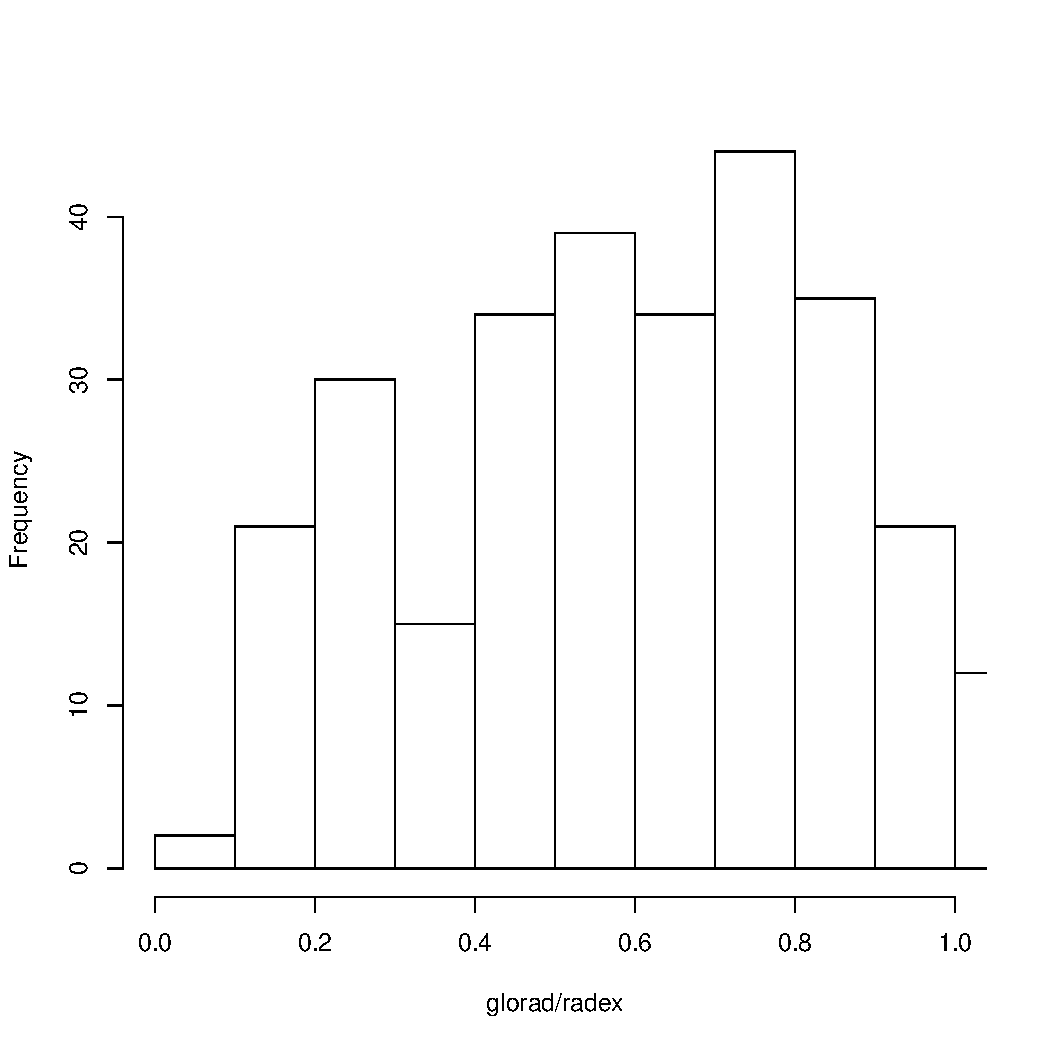
\includegraphics[width=0.5\hsize]{./plot_radex1.pdf}
  \caption{Histogram of the ratio $R_{inS}/R_{ex}$ for values less than 1 in Portugal.}
  \label{fig:portugal_radex1}
\end{figure}

\begin{figure}[ht]
  \centering
  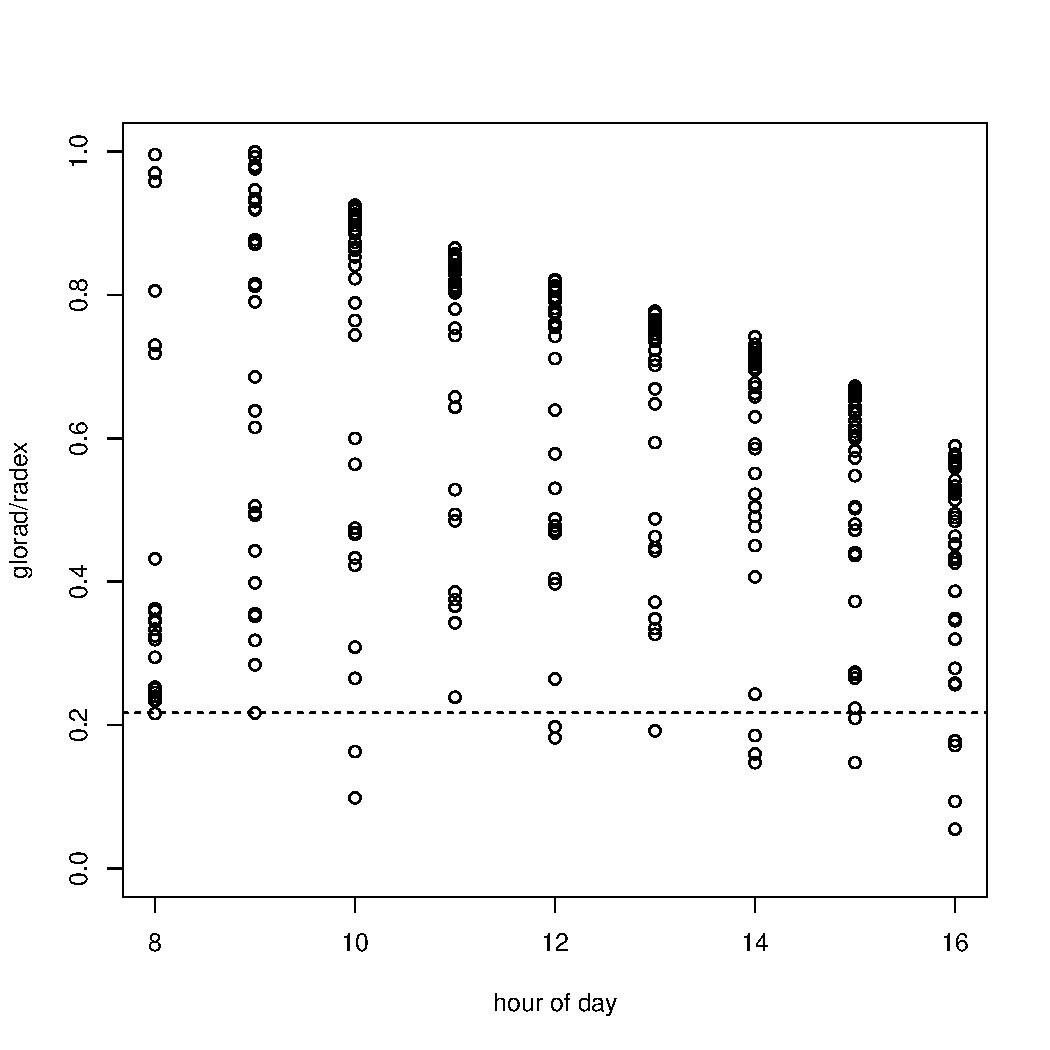
\includegraphics[width=0.6\hsize]{./plot_radex2.pdf}
  \caption{$R_{inS}/R_{ex}$ ratio dependent on hour of day.
           The shift of higher values toward early hours may indicate either a small temporal deviation between the simulated and the actual $R_{ex}$, or a local effect that weakens $R_{inS}$ during afternoon, or both.
           The dashed line marks the 5-percentile of the total distribution.}
  \label{fig:portugal_radex2}
\end{figure}

\subsection{\texttt{radex\_a}, \texttt{radex\_b}: Morocco} \label{ssec:parest_rad_radexmorocco}

\section{Soil hydraulic parameters} \label{sec:parest_soil}

\verb!wc_sat!, \verb!wc_res!, \verb!wc_pwp!, \verb!wc_etmax!, \verb!bubble!, \verb!pores_ind!, \verb!wstressmin!, \verb!wstressmax!, \verb!soil_dens!, \verb!rss_a!, \verb!rss_b!.

\section{Vegetation parameters} \label{sec:parest_veg}

\verb!ext!, \verb!par_stressHum!, \verb!crop_makk!, \verb!crop_faoref!, \verb!res_leaf_min!, \verb!lai!, \verb!cano_height!.

The Makkink crop factor \verb!crop_makk! was estimated from the leaf area index by the affine relation
\begin{align} \label{eq:cropmakk}
  \text{Makkink~crop~factor} \approx 0.14 ~ LAI + 0.4
\end{align}
%
with
\begin{itemize}
  \item[] $LAI$: leaf area index, in m$^2$ m$^{-2}$.
\end{itemize}
%
This relation was derived in the ECHSE documentation from data of \citet{feddes87} and \citet{ludwig06}.

The FAO crop factor was set to 1.
This value corresponds to the \emph{reference crop} (well-watered grass of 0.12 m height, 70 s m$^{-1}$ surface resistance, 0.23 albedo).
Since the FAO Penman-Monteith equation is just a simplification of the Penman-Monteith equation, I preferred using the original Penman-Monteith model for the study cases and using the FAO reference evaporation only for a subsumption of the different models.

%--------------------------------------------------------------------------------

\chapter{Comparison of evapotranspiration models} \label{ch:modelcomp}

%--------------------------------------------------------------------------------

\chapter{Sensitivity analysis} \label{ch:sensana}

%--------------------------------------------------------------------------------

\chapter{Evaluation of ECHSE methods} \label{ch:methodcomp}

\section{Global radiation \texttt{glorad}}

\subsection{\texttt{glorad}: Portugal}

\begin{figure}[ht]
  \centering
  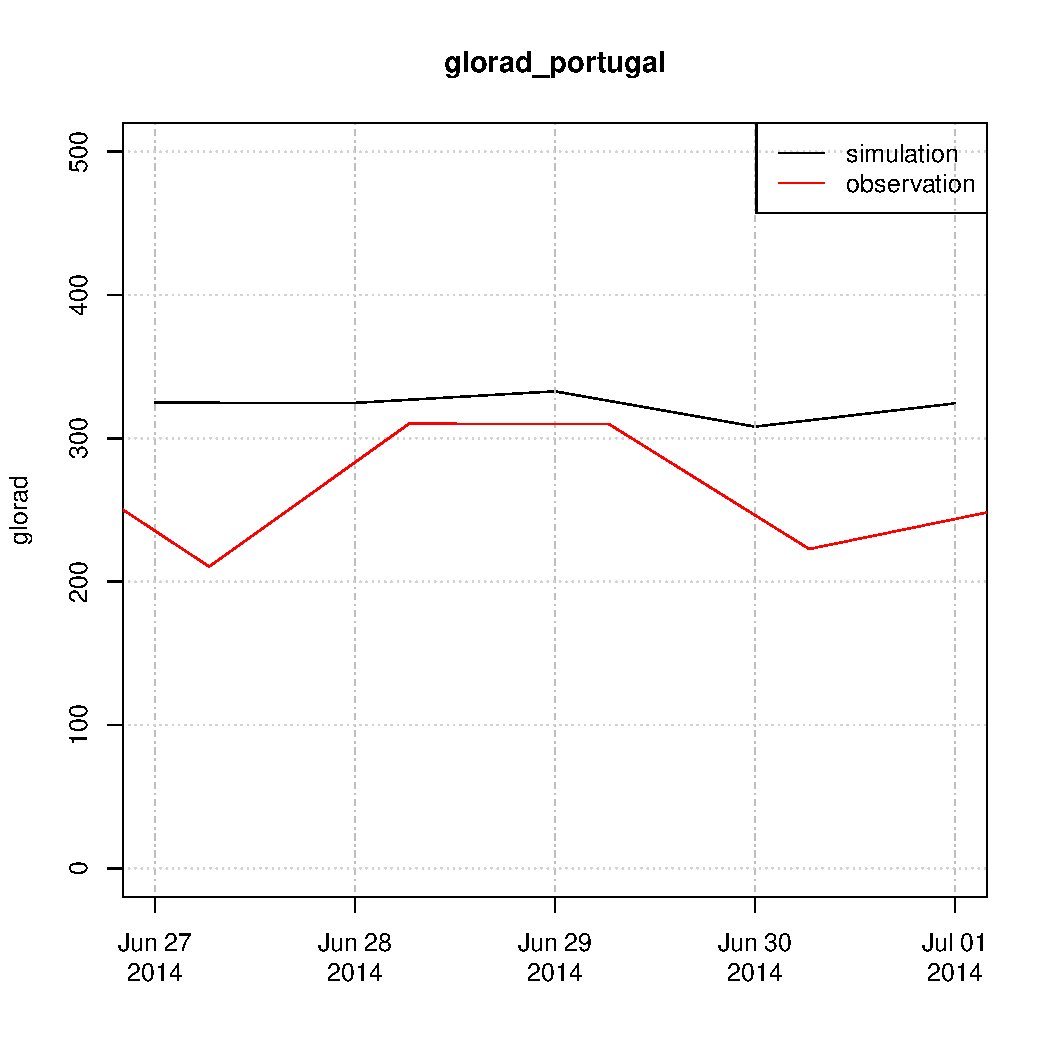
\includegraphics[width=0.8\hsize]{./plot_glorad_compare_portugal_HS_2014-06-26_2014-07-01.pdf}
  \caption{.}
  \label{fig:portugal_HS_glorad1}
\end{figure}

\begin{figure}[ht]
  \centering
  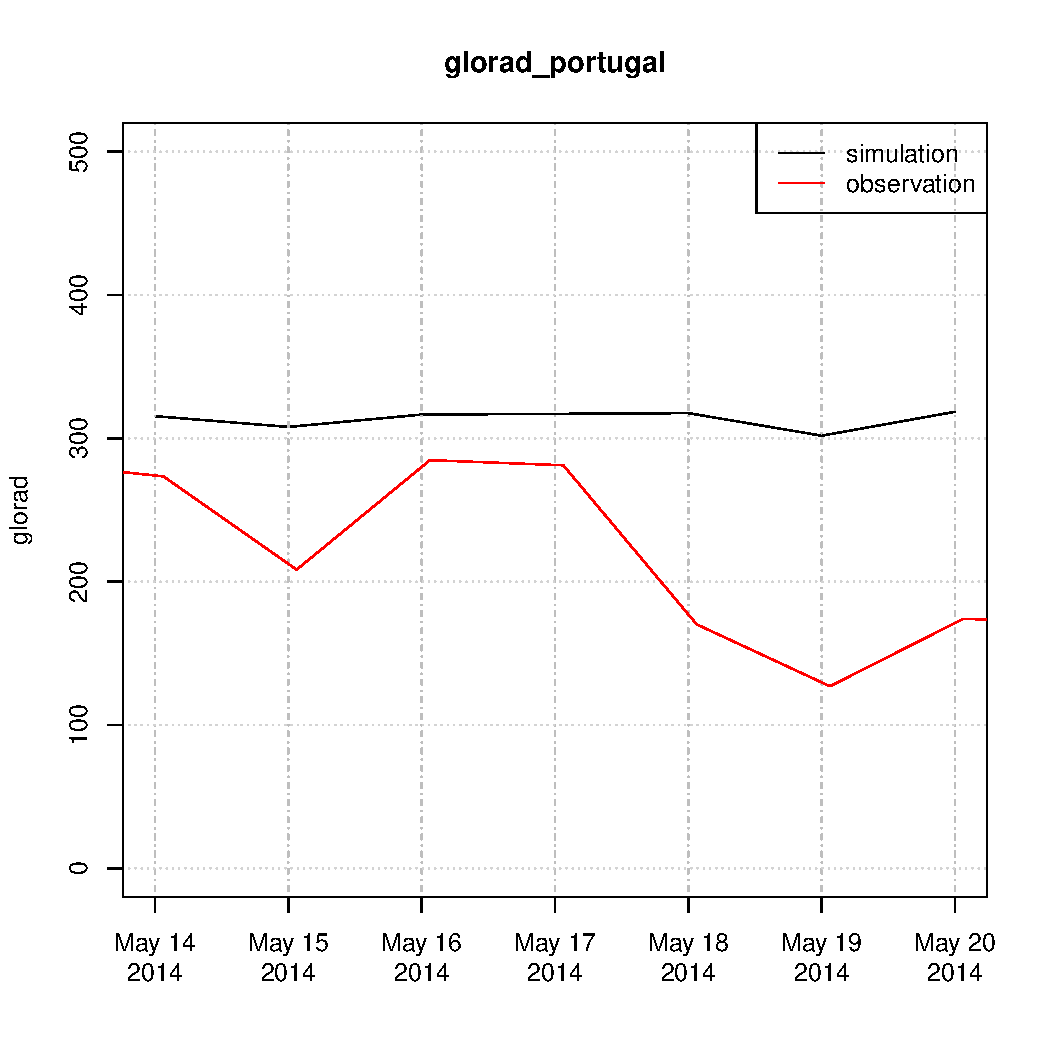
\includegraphics[width=0.8\hsize]{./plot_glorad_compare_portugal_NSA_2014-05-13_2014-05-20.pdf}
  \caption{.}
  \label{fig:portugal_NSA_glorad1}
\end{figure}

\subsection{\texttt{glorad}: Morocco}

\section{Net incoming radiation \texttt{rad\_net}}

\subsection{\texttt{rad\_net}: Portugal}

\begin{figure}[ht]
  \centering
  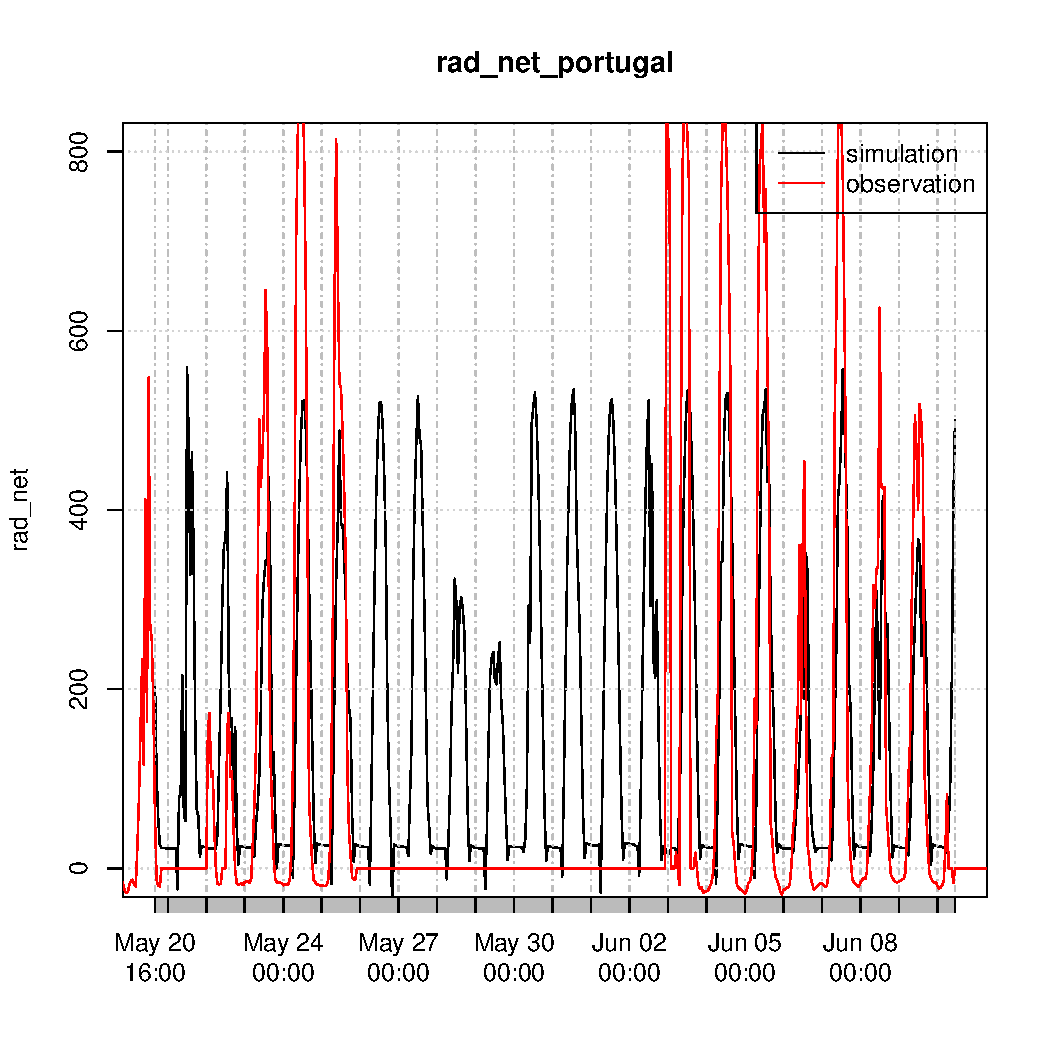
\includegraphics[width=0.8\hsize]{./plot_rad_net_compare_portugal_HS_2014-04-29_2014-07-01.pdf}
  \caption{.}
  \label{fig:portugal_HS_radnet1}
\end{figure}

\begin{figure}[ht]
  \centering
  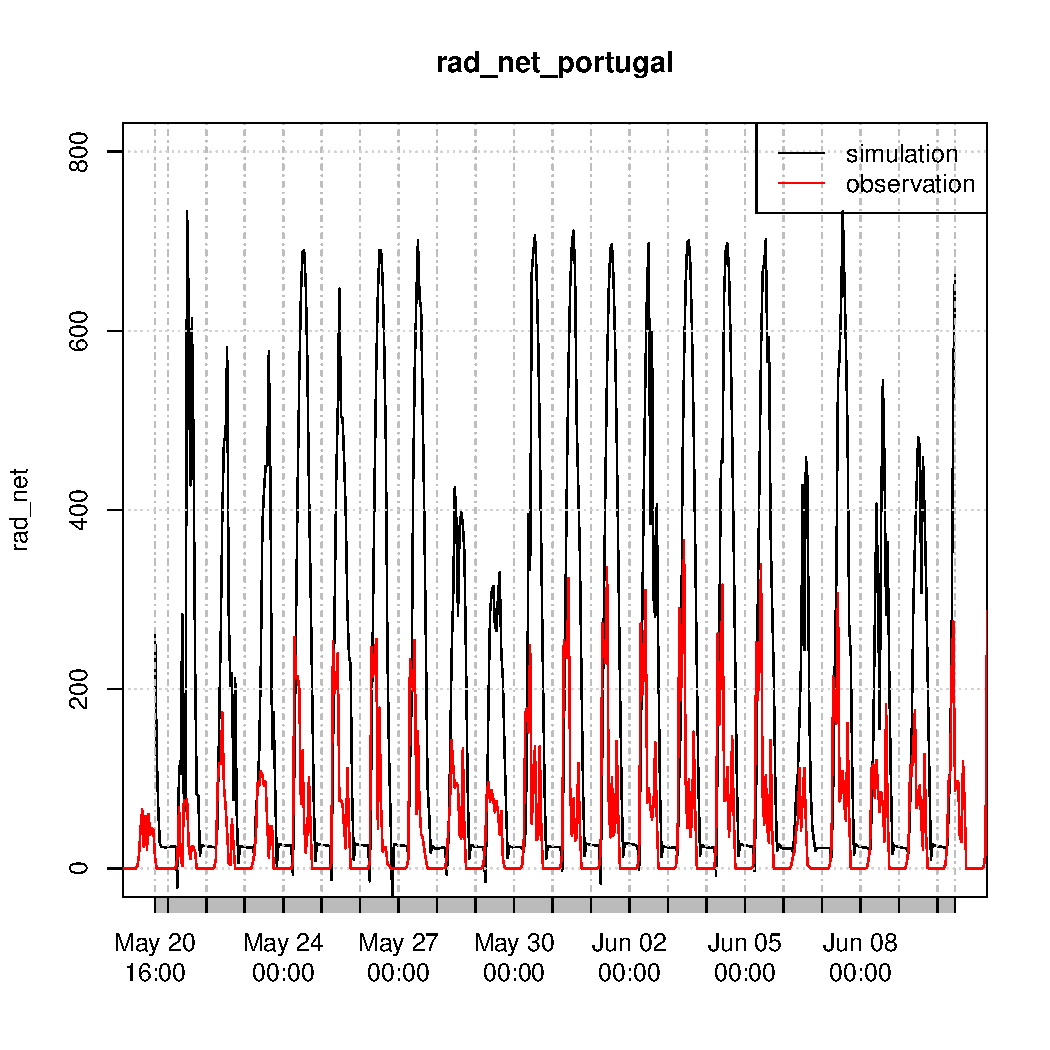
\includegraphics[width=0.8\hsize]{./plot_rad_net_compare_portugal_NSA_2014-04-29_2014-07-01.pdf}
  \caption{.}
  \label{fig:portugal_NSA_radnet1}
\end{figure}

\section{Soilheat flux \texttt{soilheat}}

\subsection{\texttt{soilheat}: Portugal}

\begin{figure}[ht]
  \centering
  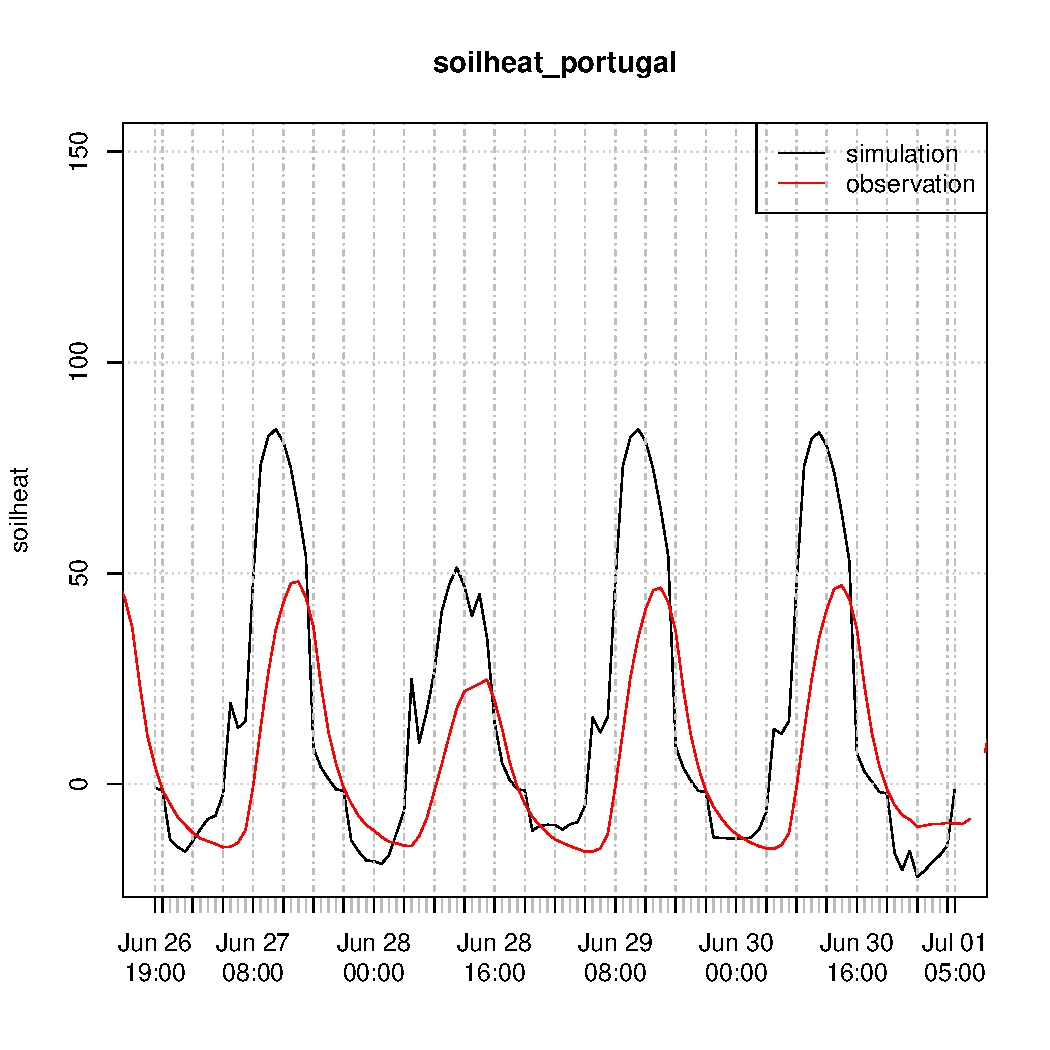
\includegraphics[width=0.8\hsize]{./plot_soilheat_compare_portugal_HS_2014-06-26_2014-07-01.pdf}
  \caption{.}
  \label{fig:portugal_HS_soilheat1}
\end{figure}

\begin{figure}[ht]
  \centering
  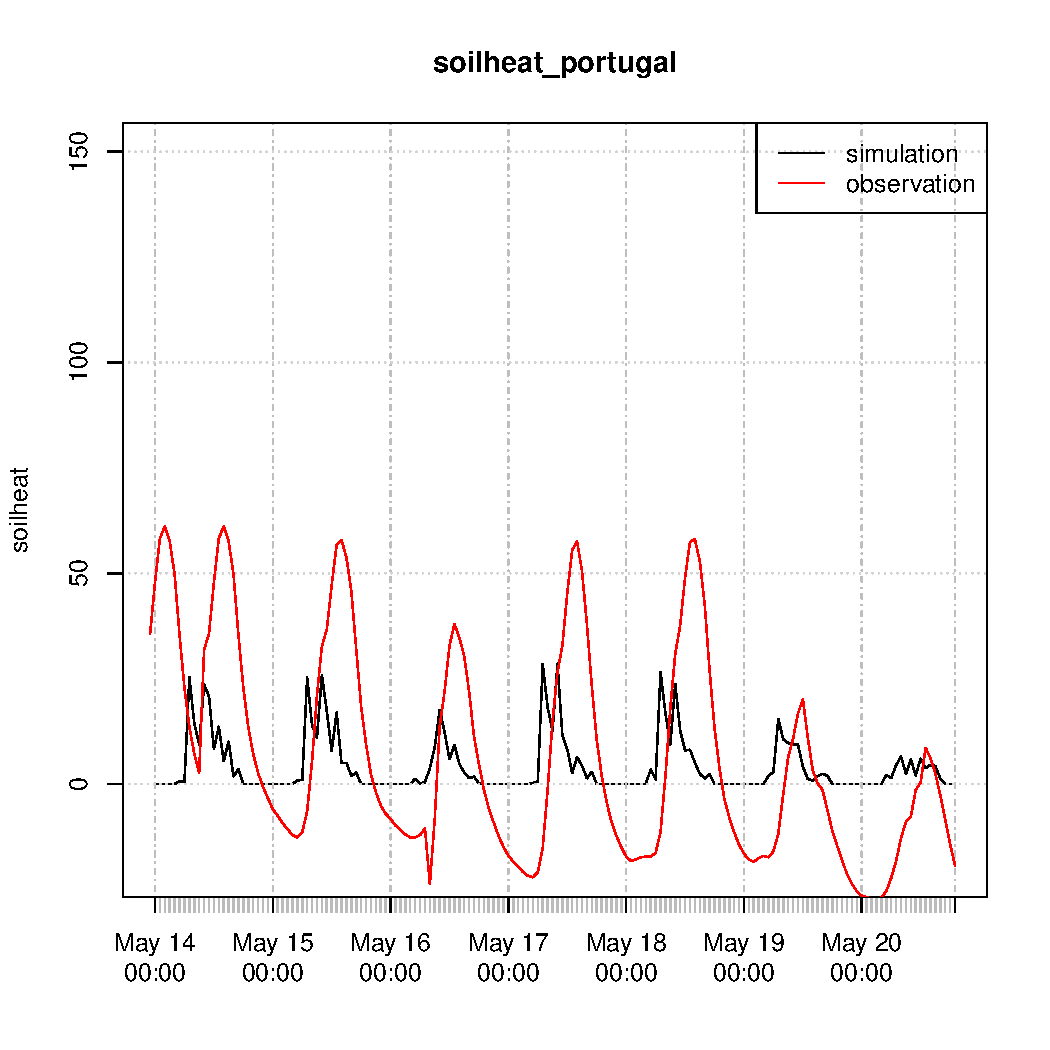
\includegraphics[width=0.8\hsize]{./plot_soilheat_compare_portugal_NSA_2014-05-13_2014-05-20.pdf}
  \caption{.}
  \label{fig:portugal_NSA_soilheat1}
\end{figure}


%--------------------------------------------------------------------------------

\chapter{Results: overview} \label{ch:results}

\section{Parameters} \label{sec:results_par}

An overview of the parameters is given for the \textsf{paramNum} group (object-specific scalar parameters, HS Portugal: Tab. \ref{tab:portugalHS_paramNum}, NSA Portugal: Tab. \ref{tab:portugalNSA_paramNum}, Morocco: Tab.), the \textsf{sharedParamNum} group (group-specific scalar parameters, HS Portugal: Tab. \ref{tab:portugalHS_sharedParamNum}, NSA Portugal: Tab. \ref{tab:portugalNSA_sharedParamNum}, Morocco: Tab.), and the \textsf{inputExt} group (group-specific scalar parameters given as time series, HS Portugal: Tab. \ref{tab:portugalHS_inputExt}, NSA Portugal: Tab. \ref{tab:portugalNSA_inputExt}, Morocco: Tab.).

% latex table generated in R 3.2.2 by xtable 1.8-2 package
% Fri May 12 11:06:02 2017
\begin{table}[ht]
\centering
\caption{Object-specific scalar parameters (\textsf{paramNum}), HS Portugal} 
\label{tab:portugalHS_paramNum}
\begin{tabular}{lrll}
  \hline
Parameter & Value & Unit & Comment \\ 
  \hline
\verb!bubble! & 8.08 & hPa & PTF by \citet{rawls85} \\ 
  \verb!crop_faoref! & 1.00 & -- & evaporation of reference crop \\ 
  \verb!crop_makk! & 0.80 & -- & Eq. \eqref{eq:cropmakk} \\ 
  \verb!elev! & 160.00 & m & local elevation map \\ 
  \verb!glo_half! & 200.00 & W m$^{-2}$ & guessed \\ 
  \verb!lat! & 39.14 & ° & GIS data \\ 
  \verb!lon! & 8.33 & ° & ditto \\ 
  \verb!par_stressHum! & 0.03 & hPa$^{-1}$ & guessed \\ 
  \verb!pores_ind! & 0.45 & -- & PTF by \citet{rawls85} \\ 
  \verb!res_leaf_min! & 50.00 & s m$^{-1}$ & guessed \\ 
  \verb!soil_dens! & 1500.00 & kg m$^{-3}$ & guessed \\ 
  \verb!wc_etmax! & 0.13 & -- & calibration \\ 
  \verb!wc_pwp! & 0.07 & -- & PTF by \citet{rawls85} \\ 
  \verb!wc_res! & 0.05 & -- & (PTF by \citet{rawls85}) \\ 
  \verb!wc_sat! & 0.39 & -- & PTF by \citet{woesten99} \\ 
  \verb!wstressmax! & 10000.00 & hPa & wilting point \\ 
  \verb!wstressmin! & 100.00 & hPa & field capacity \\ 
   \hline
\end{tabular}
\end{table}


% latex table generated in R 3.3.1 by xtable 1.8-2 package
% Fri Jun 23 13:13:45 2017
\begin{table}[ht]
\centering
\caption{Object-specific scalar parameters (\textsf{paramNum}), NSA Portugal} 
\label{tab:portugalNSA_paramNum}
\begin{tabular}{lrll}
  \hline
Parameter & Value & Unit & Comment \\ 
  \hline
\verb!bubble! & 8.08 & hPa & PTF by \citet{rawls85} \\ 
  \verb!crop_faoref! & 1.00 & -- & evaporation of reference crop \\ 
  \verb!crop_makk! & 0.51 & -- & Eq. \eqref{eq:cropmakk} \\ 
  \verb!elev! & 160.00 & m & local elevation map \\ 
  \verb!glo_half! & 200.00 & W m$^{-2}$ & guessed \\ 
  \verb!lat! & 39.14 & ° & GIS data \\ 
  \verb!lon! & 8.33 & ° & ditto \\ 
  \verb!par_stressHum! & 0.03 & hPa$^{-1}$ & guessed \\ 
  \verb!pores_ind! & 0.45 & -- & PTF by \citet{rawls85} \\ 
  \verb!res_leaf_min! & 50.00 & s m$^{-1}$ & guessed \\ 
  \verb!soil_dens! & 1500.00 & kg m$^{-3}$ & guessed \\ 
  \verb!wc_etmax! & 0.13 & -- & calibration \\ 
  \verb!wc_pwp! & 0.07 & -- & PTF by \citet{rawls85} \\ 
  \verb!wc_res! & 0.05 & -- & (PTF by \citet{rawls85}) \\ 
  \verb!wc_sat! & 0.39 & -- & PTF by \citet{woesten99} \\ 
  \verb!wstressmax! & 13100.00 & hPa & wilting point \\ 
  \verb!wstressmin! & 100.00 & hPa & field capacity \\ 
   \hline
\end{tabular}
\end{table}


% latex table generated in R 3.3.1 by xtable 1.8-2 package
% Mon Feb 13 13:53:26 2017
\begin{table}[ht]
\centering
\caption{Group-specific scalar parameters (\textsf{sharedParamNum}), HS Portugal} 
\label{tab:portugalHS_sharedParamNum}
\begin{tabular}{lrll}
  \hline
Parameter & Value & Unit & Comment \\ 
  \hline
\verb!drag_coef! & 0.07 & -- & calibration \\ 
  \verb!eddy_decay! & 2.50 & -- & as used by \citet{shuttleworth85} from \citet{monteith73} \\ 
  \verb!emis_a! & 0.34 & -- & as used by \citet{maidment93} for average conditions \\ 
  \verb!emis_b! & -0.14 & -- & ditto \\ 
  \verb!ext! & 0.40 & -- & guessed \\ 
  \verb!f_day! & 0.14 & -- & estimation from soil heat data \\ 
  \verb!f_night! & 0.49 & -- & ditto \\ 
  \verb!fcorr_a! & 1.35 & -- & as used by \citet{maidment93} \\ 
  \verb!fcorr_b! & -0.35 & -- & ditto \\ 
  \verb!h_humMeas! & 2.00 & m &  \\ 
  \verb!h_tempMeas! & 2.00 & m &  \\ 
  \verb!h_windMeas! & 2.00 & m &  \\ 
  \verb!radex_a! & 0.14 & -- & estimation from radiation data \\ 
  \verb!radex_b! & 0.67 & -- & ditto \\ 
  \verb!res_b! & 25.00 & s m$^{-1}$ & as used by \citet{shuttleworth85} \\ 
  \verb!rough_bare! & 0.01 & m & ditto \\ 
  \verb!rss_a! & 37.50 & -- &  \\ 
  \verb!rss_b! & -1.23 & -- &  \\ 
   \hline
\end{tabular}
\end{table}


% latex table generated in R 3.3.1 by xtable 1.8-2 package
% Wed Dec 14 20:44:30 2016
\begin{table}[ht]
\centering
\caption{Group-specific scalar parameters (\textsf{sharedParamNum}), NSA Portugal} 
\label{tab:portugalNSA_sharedParamNum}
\begin{tabular}{lrll}
  \hline
Parameter & Value & Unit & Comment \\ 
  \hline
\verb!drag_coef! & 0.07 & -- & calibration \\ 
  \verb!eddy_decay! & 2.50 & -- & as used by \citet{shuttleworth85} from \citet{monteith73} \\ 
  \verb!emis_a! & 0.34 & -- & as used by \citet{maidment93} for average conditions \\ 
  \verb!emis_b! & -0.14 & -- & ditto \\ 
  \verb!ext! & 0.40 & -- & guessed \\ 
  \verb!f_day! & 0.10 & -- & estimation from soil heat data \\ 
  \verb!f_night! & 0.70 & -- & ditto \\ 
  \verb!fcorr_a! & 1.35 & -- & as used by \citet{maidment93} \\ 
  \verb!fcorr_b! & -0.35 & -- & ditto \\ 
  \verb!h_humMeas! & 4.84 & m &  \\ 
  \verb!h_tempMeas! & 4.84 & m &  \\ 
  \verb!h_windMeas! & 4.84 & m &  \\ 
  \verb!radex_a! & 0.14 & -- & estimation from radiation data \\ 
  \verb!radex_b! & 0.67 & -- & ditto \\ 
  \verb!res_b! & 25.00 & s m$^{-1}$ & as used by \citet{shuttleworth85} \\ 
  \verb!rough_bare! & 0.01 & m & ditto \\ 
  \verb!rss_a! & 37.50 & -- &  \\ 
  \verb!rss_b! & -1.23 & -- &  \\ 
   \hline
\end{tabular}
\end{table}


% latex table generated in R 3.2.2 by xtable 1.8-2 package
% Fri May 19 10:20:10 2017
\begin{table}[ht]
\centering
\caption{Time-dependent parameters (\textsf{inputExt}), HS Portugal} 
\label{tab:portugalHS_inputExt}
\begin{tabular}{lrl}
  \hline
Parameter & Value & Unit \\ 
  \hline
\verb!alb! & 0.07 & -- \\ 
  \verb!cano_height! & 0.20 & m \\ 
  \verb!lai! & 0.78 & -- \\ 
   \hline
\end{tabular}
\end{table}


% latex table generated in R 3.3.1 by xtable 1.8-2 package
% Fri May 26 11:49:56 2017
\begin{table}[ht]
\centering
\caption{Time-dependent parameters (\textsf{inputExt}), NSA Portugal} 
\label{tab:portugalNSA_inputExt}
\begin{tabular}{lrl}
  \hline
Parameter & Value & Unit \\ 
  \hline
\verb!alb! & 0.07 & -- \\ 
  \verb!cano_height! & 7.98 & m \\ 
  \verb!lai! & 1.40 & -- \\ 
   \hline
\end{tabular}
\end{table}


%--------------------------------------------------------------------------------

\chapter{Conclusion} \label{ch:conclusion}

\begin{itemize}
  \item[--] Soil heat flux needs a better model.
\end{itemize}

%--------------------------------------------------------------------------------

\bibliography{../../Tex/jubib}

%--------------------------------------------------------------------------------

\end{document}